% DEFINING COLORS COF, PUR, GREEO AND GREET
\definecolor{cof}{RGB}{219,144,71}
\definecolor{pur}{RGB}{186,146,162}
\definecolor{greeo}{RGB}{91,173,69}
\definecolor{greet}{RGB}{52,111,72}
% TETRAHEDRON
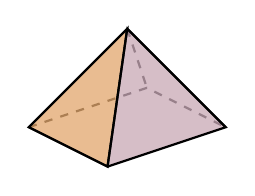
\begin{tikzpicture}[thick,scale=2.5]
    \coordinate (A1) at (0,0);
    \coordinate (A2) at (0.6,0.2);
    \coordinate (A3) at (1,0);
    \coordinate (A4) at (0.4,-0.2);
    \coordinate (B1) at (0.5,0.5);
    %
    \begin{scope}[thick,dashed,,opacity=0.6]
        \draw (A1) -- (A2) -- (A3);
        \draw (B1) -- (A2);
    \end{scope}
    \draw[fill=cof,opacity=0.6] (A1) -- (A4) -- (B1);
    \draw[fill=pur,opacity=0.6] (A4) -- (B1) -- (A3);
    %
    \draw (A1) -- (B1) -- (A4) --cycle;
    \draw (A4) -- (A3) -- (B1) ;
    %
\end{tikzpicture}
% RECTANGULAR CUBE
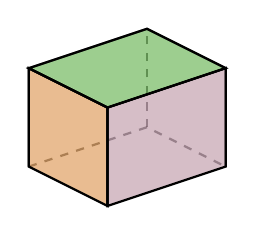
\begin{tikzpicture}[thick,scale=2.5]
    \coordinate (A1) at (0,0);
    \coordinate (A2) at (0.6,0.2);
    \coordinate (A3) at (1,0);
    \coordinate (A4) at (0.4,-0.2);
    \coordinate (B1) at (0,0.5);
    \coordinate (B2) at (0.6,0.7);
    \coordinate (B3) at (1,0.5);
    \coordinate (B4) at (0.4,0.3);
    %
    \begin{scope}[thick,dashed,,opacity=0.6]
        \draw (A1) -- (A2) -- (A3);
        \draw (A2) -- (B2);
    \end{scope}
    %
    \draw[fill=cof,opacity=0.6] (A1) -- (B1) -- (B4) -- (A4);
    \draw[fill=pur,opacity=0.6] (A4) -- (B4) -- (B3) -- (A3);
    \draw[fill=greeo,opacity=0.6] (B4) -- (B1) -- (B2) -- (B3);
    %
    \draw (A1) -- (B1) -- (B4) -- (A4) --cycle;
    \draw (A4) -- (B4) -- (B3) -- (A3) --cycle;
    \draw (B4) -- (B1) -- (B2) -- (B3) --cycle;
    %
\end{tikzpicture}
% OCTAHEDRON
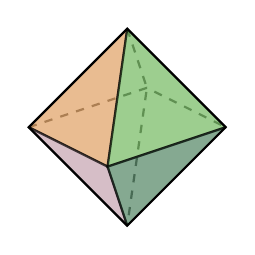
\begin{tikzpicture}[thick,scale=2.5]
    \coordinate (A1) at (0,0);
    \coordinate (A2) at (0.6,0.2);
    \coordinate (A3) at (1,0);
    \coordinate (A4) at (0.4,-0.2);
    \coordinate (B1) at (0.5,0.5);
    \coordinate (B2) at (0.5,-0.5);
    %
    \begin{scope}[thick,dashed,,opacity=0.6]
        \draw (A1) -- (A2) -- (A3);
        \draw (B1) -- (A2) -- (B2);
    \end{scope}
    %
    \draw[fill=cof,opacity=0.6] (A1) -- (A4) -- (B1);
    \draw[fill=pur,opacity=0.6] (A1) -- (A4) -- (B2);
    \draw[fill=greeo,opacity=0.6] (A3) -- (A4) -- (B1);
    \draw[fill=greet,opacity=0.6] (A3) -- (A4) -- (B2);
    \draw (B1) -- (A1) -- (B2) -- (A3) --cycle;
\end{tikzpicture}
% Prism
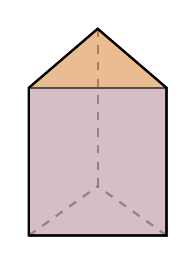
\begin{tikzpicture}[thick,scale=2.5]
    \coordinate (A1) at (0,0);
    \coordinate (A3) at (0.7,0);
    \coordinate (A4) at (0,-0.75);
    \coordinate (A5) at (0.7,-0.75);
    \coordinate (B1) at (0.35,0.3);
    \coordinate (B2) at (0.35,-0.5);
    %
    \begin{scope}[thick,dashed,opacity=0.6]
        \draw (B1)  -- (B2);
        \draw (A4) -- (B2);
        \draw (A5) -- (B2);
    \end{scope}
    %
    \draw[fill=cof,opacity=0.6] (A1) -- (B1) -- (A3);
    \draw[fill=pur,opacity=0.6] (A1) -- (A3) -- (A5) -- (A4);
    %
    \draw (A1) -- (B1) -- (A3) -- (A5) -- (A4) --cycle;
    %
\end{tikzpicture}